\documentclass[9pt]{memoir}

\input{new.tex}
\begin{document}

\titleINF

\chapter{Вступ}

\epigraph{Присвячується Маші та Міші}{}

\section{Системна інженерія та верифікація}
Протягом історії обчислювальної техніки було створено різні класи та способи обчислень,
різні тоеорії та підходи до програмування таких систем, різні класи систем програмування.
Зараз уже стало зрозумілим, що інженіринг систем які не піддаються до верифікації
формальними методами не може бути застосований у галузях де вимоги до якості
особливо підвищені, як то космонавтика, енергетика та фінанси.

\paragraph{}
Об'єктом дослідження данної роботи є системи верифікації програмного забезпечення
та операційні системи яки виконують
обчислення в реальному часі, їх поєднання та побудова формальної системи для
унифікованого середовища, яке поєднує середовище виконання та систему верифікації у єдину систему мов.
Розрізняють наступні класи систем верифікації (систем доведення теорем, або пруверів):
1) автоматизовані системи, які зосереджені на максимальній автоматизації процесу доведення (Z3, HOL, Coq);
2) системи програмування з конвертацією доведених програм в довільні мови (Idris, F*, Coq);
3) логічні фреймворки зі спеціальними логічними мовами для верифікації інших мов (Twelf, TLA+, NuPRL).

\paragraph{}
Предметом дослідження такої системи мов є теорія типів, яка вивчає обчислювальні властивості мов.
Теорія типів виділилася в окрему науку Пером Мартіном-Льофом як запит на вакантне місце у
трикутнику теорій, які відповідають ізоморфізму Каррі-Говарда-Ламбека (Логіки, Мови, Категорії).
Інші дві це: теорія категорій та логіка вищих порядків. Сама система доведення теорем є
логікою. Імплементація мови програмування,
яка релізує логічну семантику здійснюється завдяки теорії типів. Формалізація методів
відбувається завдяки теорії категорій, яка є абстрактною алгеброю фунцій,
метематичним інструментом для формалізації мов програмування та довільних
математичних теорій які описуються логіками вищих порядків.

\section{Історія систем верифікації}

\paragraph{}
Перші спроби пошуку формального фундаменту для теорії обчислень були покладені
Алонзо Черчем та Хаскелем Каррі у 30-х роках 20-го століття. Було запропоноване
лямбда числення як апарат який може замінити класичну теорію множин та її аксіоматику,
пропонуючи при цьому обчислювальну семантику. Пізніше в 1958, ця мова була втілена
у вигляді LISP лауреатом премії тюрінга Джоном МакКарті, який працював в Прінстоні.
Ця мова була побудована на конструктивних примітивах, які пізніше виявилися компонентами
індуктивних конструкцій та були формалізовані за допомогою
теорії категорій Вільяма Лавіра. Окрім LISP, нетипізоване лямбда числення
маніфестується у такі мови як Erlang, JavaScript, Python.
До цих пір нетипізоване лямбла числення є одною з мов у які робиться
конвертація доведених программ (екстракція).

\paragraph{}
Перший математичний прувер AUTOMATH (і його модифікації AUT-68 та AUT-QE),
який був написаний для комп'ютерів розроблявся під керівництвом де Брейна, 1967.
У цьому прувері був квантор загальності та лямбда функція, таким чином це був перший прувер
побудрваний на засадах ізоморфізма Каррі-Говарда-Ламбека.

\paragraph{}
ML/LCF або метамова і логіка обчисльювальних функцій був наступник крок до
осягнення фундаментальної мови простору, тут впреше з'явилися алебраїчні типи даних
у вигляді індуктивних типів, поліноміальних функторів або терміновані (well-founded) дерев.
Роберт Мілнер, асистований Морісом та Н'юві розробив Метамову (ML), як
інструмент для побудови прувера LCF. LCF був основоположником у родині пруверів
HOL88, HOL90, HOL98 та останньої версії на даний час HOL/Isabell.
Пізніше були побувані категорні моделі Татсоя Хагіно (CPL, Японія)
то Робін Кокетом (Charity, Канада).

\paragraph{}
У 80-90 роках були створені інші системи автоматичного доведення теорем,
такі як Mizar (Трибулєк, 1989). PVS (Оур, Рушбі, Шанкар, 1995),
ACL2 на базі Common Lisp (Боєр, Кауфман, Мур, 1996), Otter (МакКюн, 1996).

\newpage
\section{Методи верифікації}

\paragraph{}
Можна виділити два підходи до верифікації. Перший застосовується де вже є
певна програма написана на певній мові програмування і потрібно довести ізоморфність
цієї програми до доведеної моделі. Ця задача вирішується у побудові теоретичної моделі
для певної мови програмування, потім програма на цій мові переводиться у цю
теоретичну модель і доводить ізоморфізм цієї програми у побудованій моделі до доведеної моделі.
Приклади таких систем та піходів. VST (CompCert, сертифікація C програм),
NuPRL (Cornell University, розподілені системи, залежні типи),
TLA+ (Microsoft Reseach, Леслі Лампорт), Twelf (для верифікації мов програмування).

\paragraph{}
Інший підхід можна назвати підходом вбудованих DSL. Усе моделювання відбувається
в основній мові, а сертифіковані програми автоматично екстрагуються в довільні мови.
Приклади таких систем: Coq побудована на мові OCaml від науково-дослідного
інституту Франції INRIA; Agda побудовані на мові Haskell від шведського інституту технологій Чалмерс;
Lean побудована на мові C++ від Microsoft Research та Універсистету Каргені-Мелона;
Idris подудована на мові Haskell Едвіна Бреді з шотландського Університету ім. св. Андрія;
F* -- окремий проект Microsoft Research.

\paragraph{}
Завдання цього дослідження є побудова єдиної системи, яка поєднує середовище
викодання та систему верифікації програмного забезпечення. Це прикладне дослідження,
яке є сплавом фундаментальної математики та інженерних систем з формальними методами верицікації.

\newpage
\section{Метематичне забезпечення}
\vspace{0.3cm}

\subsection{Інтуіціоністична теорія типів Мартіна-Льофа}
Пер Мартін-Льоф в 1972 році запропонував $\Pi$, $\Sigma$ та $Id$
у якості основних фундаментальних типів. З тих пір усі сучасні системи типів
для пруверів побувані наслідуючи цю модель (MLTT, теорія типів Мартіна-Льофа).
Було показано, що мова такої системи
типів є внутрішнією мовою локальних декартово-замкнених категорій. $\Pi$ та $\Sigma$
кодують безпосереднь логічні кванторти $\forall$ та $\exists$, а тип $\rightarrow$ є
частковим випадком $\Pi$-типу, коли вираз $B$ не залежить від $x$.

\paragraph{}
Аксіоми:
\begin{equation}
\tag{$\Pi$}
\dfrac{\Gamma\ x:A \vdash B : Type\ \ \ \Gamma\ \vdash A : Type}
      {\Gamma\ \vdash \Pi (x : A) \rightarrow B (x) : Type}
\end{equation}

\begin{equation}
\tag{$\Sigma$}
\dfrac{\Gamma\ x:A \vdash B : Type\ \ \ \Gamma\ \vdash A : Type}
      {\Gamma\ \vdash \Sigma (x : A) \times B (x) : Type}
\end{equation}

\begin{equation}
\tag{$Id$}
\dfrac{\Gamma\ \vdash a: A\ \ \ \ \Gamma\ \vdash b: A\ \ \ \ \Gamma\ \vdash A : Type }
      {\Gamma\ \vdash Id_A (a,b)}
\end{equation}

Теореми:
\begin{center}
\begin{tabular}{lll}
  рефлексивність &:& $Id_A(a,a)$ \\
  підстановка    &:& $Id_A(a,a') \rightarrow B(x=a) \rightarrow B(x=a')$ \\
  симетричність  &:& $Id_A(a,b) \rightarrow Id_A(b,a)$  \\
  транзитивність &:& $Id_A(a,b) \rightarrow Id_A(b,c) \rightarrow Id_A(a,c)$ \\
  конгруентність &:& $(f: A \rightarrow B) \rightarrow Id_A(x,x') \rightarrow Id_B(f(x),f(x'))$ \\
\end{tabular}
\end{center}


\newpage
\subsection{Теорія категорій}

\paragraph{}
Теорія категорій широко застосовується як інструмент для математиків у тому числі і
при аналізі програмного забезпечення. Теорію категорій можна вважати абстрактною алгеброю функцій.
Дамо конструктивне визначення категорії.
Категорії (програми) визначаються переліком своїх об’єктів (типів) та своїх
морфізмів (функцій), а також бінарною операцією композиції,
що задовольняє закону асоціативності, та з тотожнім морфізмом (тотжньою функцією --- одиницею) який існує
для кожного об’єкту (типу) категорії. Аксіоми формації об’єктів не
приводяться та авто-постулуються в нижніх аксіомах.
Поки що тут буде визначатися тільки композиція морфізмів. Об’єкти $A$ та $B$ морфізма $f: A \rightarrow B$
називаються домен та кодомен відповідно. Композиція є фундаментальною властивістю морфізмів.

\paragraph{}
Інтро аксіоми -- асоціативність композиції та права і ліва композиції одниці показують,
що категорії є типизованими моноїдами, що складаються з морфізмів та операції композиції.
Є різні мови, у тому числі і графічні, представлення категорної семантики, однак у цій роботі
ми будемо використовувати теоретико-логічні формулювання.

\paragraph{}
Аксіоми:
\vspace{-0.5cm}
\begin{fullwidth}[width=\linewidth+3cm]
\hspace{-2cm}
\parbox[t][][l]{0.60\textwidth}{
\begin{prooftree}
\AxiomC{$\Gamma\ \vdash f: A \rightarrow B$ }
\AxiomC{$\Gamma\ \vdash g: B \rightarrow C$ }
\BinaryInfC{$\Gamma \vdash g \circ f : A \rightarrow C $}
\end{prooftree}

\begin{prooftree}
\AxiomC{$\Gamma \vdash f : B \rightarrow A$ }
\AxiomC{$\Gamma \vdash g : C \rightarrow B$ }
\AxiomC{$\Gamma \vdash h : D \rightarrow C$ }
\TrinaryInfC{$\Gamma \vdash (f \circ g) \circ h = f \circ (g \circ h) : D \rightarrow A $}
\end{prooftree}

}
\hspace{0.1cm}
\parbox[t][][r]{0.40\textwidth}{

\begin{prooftree}
\AxiomC{$$ }
\UnaryInfC{$\Gamma \vdash id_A : A \rightarrow A $}
\end{prooftree}

\begin{prooftree}
\AxiomC{$\Gamma\ \vdash f: A \rightarrow B$ }
\UnaryInfC{$\Gamma \vdash f \circ id_A = f : A \rightarrow B$}
\end{prooftree}

\begin{prooftree}
\AxiomC{$\Gamma\ \vdash f: A \rightarrow B$ }
\UnaryInfC{$\Gamma \vdash id_B \circ f = f : A \rightarrow B $}
\end{prooftree}

}

\end{fullwidth}
%Теореми:
%\begin{center}
%$(f \circ g) \circ h = f \circ (g \circ h)$\\
%$A \implies id : A \rightarrow A$\\
%$f \circ id = f$\\
%$id \circ f = f$\\
%\end{center}

\newpage
\subsection{Алгебраїчні типи даних}

Після операції композиції, як способу конструювання нових об’єктів
за допомогою морфізмів далі йде операція конструювання добутка двох об’єктів певної категорії,
разом з добутком морфізмів зі спільним доменом, необхідних для визначення декартового добутка $A \times B$.

\paragraph{}
Це є внутрішня мова декартової категорії, у якій для будь яких двох доменів існує їх декартова сума (кодобутку)
та декартовий добуток (косума, кортеж), за допомогою яких конструюються суми-протоколи та добутки-повідмоення,
а також існує $\bot$ тип-термінал, та $\top$ тип-котермінал. Термінальними типами зручно термінувати рекурсивні
типи даних, такі як списки. Ми будемо розглядати тільки категорії які маються добутки та суми.

\paragraph{}
Добуток має природні елімінатори $\pi$ зі спільним доменом, які є морфізмами-проекціями об’єктів добутка. Сума має оберненені
елімінатори $\sigma$ зі спільним кодоменом. Як видно добуток є дуальний до суми з точністю до направлення стрілок,
таким чином елімінатори $\pi$ та $\sigma$ є оберненими, тобто $\pi \circ \sigma = \sigma \circ \pi = id$.

\paragraph{}
Аксіоми:
\vspace{-0.5cm}
\begin{fullwidth}[width=\linewidth+2cm]
\hspace{-0.5cm}
\parbox[t][][l]{0.50\textwidth}{

\begin{prooftree}
\AxiomC{$\Gamma \vdash\ f:A \rightarrow B$ }
\AxiomC{$\Gamma \vdash\ g:A \rightarrow C$ }
\AxiomC{$\Gamma \vdash\ B \times C$ }
\TrinaryInfC{$\Gamma \vdash\ \langle f,g \rangle : A \rightarrow B \times C$ }
\end{prooftree}

\begin{prooftree}
\AxiomC{$\Gamma\ x: A \times B$ }
\UnaryInfC{$\Gamma \vdash \pi_1\ : A \times B \rightarrow A$;
           $\Gamma \vdash \pi_2\ : A \times B \rightarrow B$}
\end{prooftree}

\begin{prooftree}
\AxiomC{$\Gamma \vdash\  a:A$ }
\AxiomC{$\Gamma \vdash\  b:B$ }
\BinaryInfC{$\Gamma \vdash\ (a,b) : A \times B$ }
\end{prooftree}

\begin{prooftree}
\AxiomC{}
\UnaryInfC{$\Gamma \vdash\ \bot$ }
\end{prooftree}

}
\hspace{0cm}
\parbox[t][][r]{0.50\textwidth}{

\begin{prooftree}
\AxiomC{}
\UnaryInfC{$\Gamma \vdash\ \top$ }
\end{prooftree}

\begin{prooftree}
\AxiomC{$\Gamma \vdash\ a:A$ }
\AxiomC{$\Gamma \vdash\ b:B$ }
\BinaryInfC{$\Gamma\vdash a\ |\ b : A + B$}
\end{prooftree}

\begin{prooftree}
\AxiomC{$\Gamma\ x: A + B$ }
\UnaryInfC{$\Gamma \vdash \sigma_1: A \rightarrow A + B$;
           $\Gamma \vdash \sigma_2: B \rightarrow A + B$}
\end{prooftree}

\begin{prooftree}
\AxiomC{$\Gamma \vdash\ f:A \rightarrow B$ }
\AxiomC{$\Gamma \vdash\ g:A \rightarrow C$ }
\AxiomC{$\Gamma \vdash\ B + C$ }
\TrinaryInfC{$\Gamma \vdash\ [f,g] : A \rightarrow B + C$ }
\end{prooftree}
}
\end{fullwidth}
    Теореми:
\begin{fullwidth}[width=\linewidth+2cm]
\parbox[t][][l]{0.5\textwidth}{
$(f \circ g) \circ h = f \circ (g \circ h)$\\
$f \circ id = f$\\
$id \circ f = f$\\
$\pi_1 \circ \langle f, g \rangle = f$
}
%\hspace{-3cm}
\vspace{-1cm}
\parbox[t][][r]{0.4\textwidth}{
$\pi_2 \circ \langle f, g \rangle = g$\\
$\langle f \circ \pi_1, f \circ \pi_2 \rangle = f$\\
$\langle f, g \rangle \circ h = \langle f \circ h, g \circ h \rangle$\\
$\langle \pi_1, \pi_2 \rangle = id$
}
\end{fullwidth}

\newpage

\subsection{Лямбда числення}
Будучи внутрішньою мовою декартово-замкненої категорії лямбда числення окрім змінних
та констант у вигляді термів пропонує операції абстракції та аплікації, що визначає
достатньо лаконічну та потужну структуру обчислень з функціями вищих порядків,
та метатипизаціями, такими як System F, яка була запропонована
вперше Робіном Мілнером в мові ML, та зараз присутня в більш складних типоих системах,
таких як System F$\omega$, та системах Haskell та Scala.

\paragraph{}
З категоріальнї точки зору експоненти $f : A^B$ є аналогами
фукціональних просторів $f: B \rightarrow A$.
Так як ми вже визначили добутки та термінали, то ми можемо визначити і експоненти,
опускаючи усі категоріальні подробиці ми визначимо конструювання функції (операція абстракції),
яка параметризується змінною $x$ у середовищі $\Gamma$; та її елімінатора -- операції аплікації
функції до аргументу. Так визначаєьтся декартово-замкнена категорія.
Визначається також рекурсивний механізм виклику функції
з довільною кількістю аргументів.


\begin{fullwidth}
\hspace{-2cm}
\begingroup
\parbox[t][][l]{0.40\textwidth}{

Аксіоми:

\begin{prooftree}
\AxiomC{$\Gamma\ x:A \vdash M : B$}
\UnaryInfC{$\Gamma \vdash \lambda\ x\ .\ M : A \rightarrow B$}
\end{prooftree}

\begin{prooftree}
\AxiomC{$\Gamma\ f:A \rightarrow B$ }
\AxiomC{$\Gamma\ a:A$ }
\BinaryInfC{$\Gamma \vdash apply\ f\ a\ : (A \rightarrow B) \times A \rightarrow B$}
\end{prooftree}

\begin{prooftree}
\AxiomC{$\Gamma \vdash f: A \times B \rightarrow C$ }
\UnaryInfC{$\Gamma \vdash curry\ f : A \rightarrow (B \rightarrow C)$}
\end{prooftree}

}
\hspace{1cm}
\parbox[t][][r]{0.60\textwidth}{

Теореми:

\begin{center}
$apply \circ \langle (curry\ f) \circ \pi_1 , \pi_2 \rangle = f$\\
$curry\ apply \circ \langle g \circ \pi_1, \pi_2 \rangle) = g$\\
$apply \circ \langle curry\ f, g \rangle = f \circ \langle id , g\rangle$\\
$(curry\ f) \circ g = curry\ (f \circ \langle g \circ \pi_1,\pi_2\rangle)$\\
$curry\ apply = id$\\
\end{center}
}
\endgroup
\end{fullwidth}

\begin{center}
Об’єкти : $\top$\ |\ $\bot\ |\ \rightarrow\ |\ \times\ |\ +$\\
Морфізми : $id\ |\ f \circ g\ |\ [f,g]\ |\ \langle f, g \rangle\ |\ apply\ |\ \lambda\ |\ curry$
\end{center}

\newpage
\subsection{Індуктивні типи}
Системи з залежними типами як верифікаційні математичні формальні моделі
для доведення корректності. Система $\Sigma$ та $\Pi$ типів, як кванторів
існування та узагальнення. Системи Mizar, Coq, Agda, Idris, F*, Lean. Ми будемо
використовувати cubicaltt, Coq та Lean для доведення MLTT моделей.

\paragraph{}
Розбудовуючи певний фреймворк чи систему конструктивними методами
так чи інакше доведеться зробити певний вибір у мові та способі кодування.
Так при розробці теорії абстрактної алгебри в Coq були використані
поліморфні індуктивні структури. Однак Agda та Idris використувують
для побудови алгебраїчної теорії типи класів, а у Idris взагалі відсутні
поліморфірні індуктивні структури та коіндуктивні структури. В Lean
теж відсутні коіндуктивні структури проте повністю реалізована теорія
HoTT на нерекурсивних поліморфних структурах що обєднує основні чотири
класи математичних теорій: логіка, топологія, теорія множин, теорія типів.
Як було показано Стефаном Касом, одна з стратегій імплементації типів
класів --- це використання поліморфних структур.

\begin{equation}
\tag{$W$-formation}
\dfrac{A:Type\ \ \ \ x:A\ \ \ \ B(x):Type}
      {W (x:A) \rightarrow B(x) : Type}
\end{equation}

\begin{equation}
\tag{$W$-intro}
\dfrac{a:A\ \ \ \ t: B(a) \rightarrow W}
      {sup(a,t) : W}
\end{equation}

\begin{equation}
\tag{$W$-elimination}
\dfrac{w: W \vdash C(w) : Type\ \ \ \ x:A,\ u:B(x) \rightarrow W,\ \ \ \ v:\Pi (y:B(x)) \rightarrow C(u(y)) \vdash c(x,u,v):C(sup(x,u))}
      {w:W \vdash wrec(w,c):C(w)}
\end{equation}

\newpage
    \subsection{Числення процесів}
    Теорія $\pi$-числення процесів Роберта Мілнера є основним формалізмом обчислювальної
    теорії розподілених систем та її імплементації. З часів виникнення CSP числення розробленого Хоаром,
    Мілнеру вдалося значно розширити та адаптувати теорію до сучасних
    телекомунікаційних вимог, як наприклад хендовери в мобільних мережах.
    Основні теорми в моделі $\pi$-числення стосуються непротиречивості та неблокованості
    у синхронному виконанні мобільних процесів. Так як сучасний Web можно розглядати
    як телекомунікаційну систему, тому у розробці додатків можна покладатися у тому
    числі і на такі моделі як $\pi$-числення.
    Також ми анонсуємо процес як фундаменльний тип даних, подібний до функції але який здатний
    тримати певний стан у вигляді типа коротежа та є морфізмом-одиницею типу свого стану.

\begin{prooftree}
\AxiomC{$\Gamma\ \vdash E, \Sigma, X$ }
\AxiomC{$\Gamma\ \vdash action : \Sigma \times X \rightarrow \Sigma \times X$ }
\BinaryInfC{$\Gamma \vdash {spawn}\ action : \pi_\Sigma $}
\end{prooftree}

\begin{prooftree}
\AxiomC{$\Gamma\ \vdash pid : \pi_\Sigma$ }
\AxiomC{$\Gamma\ \vdash msg : \Sigma$ }
\BinaryInfC{$\Gamma \vdash join\ msg\ pid : \Sigma \times \pi_\Sigma \xrightarrow{\bullet} \Sigma$;
            $\Gamma \vdash send\ msg\ pid : \Sigma \times \pi_\Sigma \rightarrow \Sigma$}
\end{prooftree}

\begin{prooftree}
\AxiomC{$\Gamma\ \vdash L : A + B, R : X + Y$ }
\AxiomC{$\Gamma\ \vdash M : A \rightarrow X, N : B \rightarrow Y$ }
\BinaryInfC{$\Gamma \vdash receive\ L\ M\ N : L \xrightarrow{\bullet} R$}
\end{prooftree}
\paragraph{}

    \paragraph{}
    Алгебра процесів визначає базові операції мультиплексування двох чи декількох
    протоколів в рамках одного процесу (добуток), а також паралельного запуску процесів (сума).

\begin{center}
\begin{tabular}{lcl}
$\oplus$   &:& $\pi \parallel \pi$\\
$\otimes$  &:& $\pi \mid \pi$\\
\end{tabular}
\end{center}

\newpage
\section{Дослідження систем типів}
Головна ідея цієї роботи -- побудова гнучкої сучасної мови,
яка здатна була би обслуговувати академію та виробництво,
тобто у якій можно було би створювати моделі, тут же у цій мові їх доводити,
та екстрагувати код через оптимізоване ядро у інтерпритатор чи мови які продукують машинний код.

\paragraph{}
Працюючи над розподіленими системами, системами зберігання даних та
системами обробки тензорних масивів, автором було виявлено глибокий
зв'язок Pi-числення процесів (Erlang, Ling) і Stream-числення для обробки
тензорних масивів (Futhark, Spiral). Тому ми почали займатися дослідженням
гнучкої типової системи яка би могла поєднувати різні моделі мов з одним
уніфокованим MLTT ядром.

\paragraph{}
В ході дослідження були виявлені основні типові системи, або мовні рівні, які
пропонується сприймати як протоколи, які можуть підключатися додаючи до
системи нові мовні рівні.

\subsection{PTS системи}
З тих часів, як Кокуанд відкрив числення конструкцій, та Берендрехт систематизував його варіації,
теорія чистих типових систем (Pure Type Systems, PTS) стала вже достатньо розробленою.
Також вона відома як теорія з одніє аксіомою --- $\Pi$-типом MLTT теорії без $\Sigma$ та $Id$ типа. Ця теорія репрезентую функціональну повноту
згідно Герміди-Якобса.

\begin{lstlisting}[mathescape=true]
name: U = list nat

data $O_1$ = star (n: nat)
         | var (n: name)
         | app (f a: $O_1$)
         | lambda (x: name) (d c: $O_1$)
         | arrow (d c: $O_1$)
         | pi (x: name) (d c: $O_1$)
\end{lstlisting}

Такі системи є простими, проте зрозумілими та досить потужними, аби реалізувати на такій системі
системі $System F$ бібліотеку. Нами була вибрана система $PTS_{\infty}$,
яка підтримує нескінченну кількість всесвітів, що унеможливлює парадокси Хуркенса-Рассела-Жирара
і має два режими: предикативний та імпредикативний. Ця система типів представлена
у нашій роботі як мова $Om$, яка виступає ядром системи доведення, верифікації та екстрагування.

\newpage
\subsection{MLTT системи}
Для доведення теорем необхіден $\Sigma$-тип, а також рівність на твердженнях.
Саме тому теорія типів Мартіна-Льофа з самого початку була облаштова цими конструціями.
В MLTT $\Sigma$-тип репрезентує контекстуальну повноту згідно Герміди-Якобса.
$\Sigma$-тип необхідний також для моделювання алгебраїчних структур-носіїв.

\begin{lstlisting}[mathescape=true]
data $O_2$ = $O_1$
         | sigma (n: name) (a b: $O_2$)
         | pair (a b: $O_2$)
         | fst (p: $O_2$)
         | snd (p: $O_2$)

data $O_3$ = $O_2$
         | id (a b: $O_3$)
         | idPair (a b: $O_3$)
         | idJ (a b c d e: $O_3$)
\end{lstlisting}

\subsection{Індуктивні системи}
В процесі глибшого дослідження індукції в MLTT теорії виникла теорія індуктивних типів,
поліноміальних функторів у застосуванні до теорії типів (або рекурсивних дерев
з визначеною базою рекурсії, W-типи). В мовах програмування вони відомі як data типи.
Насправді індуктивні типи можуть бути закодовані в PTS системах за допомогою
кодування Черча-Бома-Берардуччі, або в інших системах кодувань (Парігот, Скот, CPS, Ламбек).
Рекурсивні дерева без бази рекурсії називаються ко-індуктивними типами, та
часто можуть бути представлені як record типи, або рекурсивні record типи.

\begin{lstlisting}[mathescape=true]
data tele   (A: U) = nil | tel (n: name) (b: A) (xs: tele A)
data branch (A: U) =        br (n: name) (a: list name) (t: A)
data label  (A: U) =       lab (n: name) (t: tele A)

data $O_4$ = $O_3$
         | sum  (n: name) (t: tele $O_4$) (labels:      list (label $O_4$))
         | case (n: name) (t: ind)      (branches: list (branch $O_4$))
         | ctor (n: name)               (args:     list $O_4$)
\end{lstlisting}

\newpage
\subsection{HTS системи}
Багаточисельні фундаменальні дослідження рівності в MLTT теорії привели
до тактування $\infinity-групоїдів$ як топологічних просторів. Так в чекарах
виник $Path$-тип, розширений багатовимірний варінт $Id$-типу з оригінальної теорії Мартіна-Льофа.
Це тип моделює відрізок $[0,1]$ разом з алгеброю де Морана на цьому інтервалі.
Ця система типів необхідна для доведення гомотопічних теорем та при роботі з
вищими індуктивними типами, за домогою яких кодуються топологічні об'єкти:
багатовимірник відрізок, багатовимірна сфера, топологічні операції.
Такі системи типів називаються гомотопічними (Homotopy Type System, HTS)
та вперше були запропоновані Воєводським.

\begin{lstlisting}[mathescape=true]
data alg = zero
         | one
         | max (a b: alg)
         | min (a b: alg)

data $O_5$ = $O_4$
         | path (a b: $O_5$)
         | pathLam (n: name) (a b: $O_5$)
         | pathApp (f: alg) (a b: $O_5$)
         | comp (a b: $O_5$)
         | fill (a b c: $O_5$)
         | glue (a b c: $O_5$)
         | glueElem (a b: $O_5$)
         | unglueElem (a b: $O_5$)
\end{lstlisting}

\subsection{Pi-числення}

\subsection{Числення алгебраїчних ефектів}

\subsection{Обробка тензорних масивів}

\newpage
\section{Дослідження середовищ виконання}

Усі середовища виконання можно умовно розділити на два класи:
1) інтерпретатори нетипізованого або просто
типізованого (рідше з більш потужними системами типів),
лямбда числення з можливими JIT оптимізаціями; та 2)
безпосередня генерація інструкцій процессора і лінкування цієї програми з
середовищем виконання що забезпечує планування ресурсів
(в цій області переважно використовується System F типізація).

\paragraph{}
До першого класу можно віндеси такі віртуалні машини та інтерпретатори як
Erlang (BEAM), JavaScript (V8), Java (HotSpot), K (Kx), PHP (HHVM), Python (PyPy), LuaJIT
та багато інших інтерпретаторів.

\paragraph{}
До другого класу можна віднести такі мови програмування: ML, OCaml, Rust,
Haskell, Pony. Часто використовується LLVM як спосіб генерації програмного коду,
однак на момент публікації статті немає промислового верифікованого LLVM генератора.
Rust використовує проміжну мову MIR над LLVM рівнем. Побудова верифікованого компілятора
для такого класу систем виходить за межі цього дослідження. Нас тут буде цікавити
лише вибір найкращого кандидата для середовижа виконання.

\paragraph{}
Нійбільш цікаві цільові платформи для виконання программ
які побудовані на основі формальних доведень для нас є OCaml (тому,
що це основна мова естракту для промислової системи доведення теорем Coq),
Rust (тому, що рантайм може бути написаний без використання сміттєзбірника),
Erlang (тому, що підтримує неблоковану семантику пі-калкулуса)
та Pony (тому, що семантика його пі-калкулуса побудована на імутабельних чергах та CAS курсорах).
У цій роботі ми зосередимося на дослідженні тьох підходів
та побудові трьох прототипів.



\newpage
\section{Продукти дослідження}

\subsection{Інтерпретатор О на Rust для L4}
Перший прототип, рантайм О -- лінивий
векторизований інтерпретатор (підтримка SSE/AVX інструкцій) та система
управління ресурсами з планувальником лінивих програм
та системою черг і CAS курсорсів у якості моделі пі-калкулуса. Розглядається також
використання ядра L4 на мові С, верифікованого за допомогою HOL/Isabell,
у якості базової операційної системи.

\subsection{Коіндукція на Coq з екстрактом в OCaml}
Другий прототип побудований на базі coq.io, що дозволяє
використовувати бібліотеки OCaml для промислового програмування в Coq.
У цій роботі ми формально показали і продемонстрували коіндуктивний шел
та вічно працюючу тотальну програму на Coq. Ця робота проводилася
в рамках дослідження системи ефектів для результуючої мови програмування.

\subsection{Екстракція в Erlang та О з ОМ}
Третій прототип -- побудова тайпчекера та ектрактора у мову Erlang та O.
Ця робота представлена у вигляді PTS тайпчекера ОМ, який вистує у ролі
проміжної мови для повної нормалізації лямбда термів. В роботі використане
нерекурсивне кодування індуктивних типів та продемонстрована теж бескінечна
тотальна программа у якості способу лінкування з підсистемою вводу-виводу
віртуальної машини Erlang.

\subsection*{Idris та PureScript разом з Erlang}
Також був досліджений спосіб естракції Erlang програм з мови програмування
Idris, розглянутий протокол передачі термів-теорем в Lean,
та екстракція з PureScript в Erlang.


\newpage
\section{Структура роботи}

\begin{center}
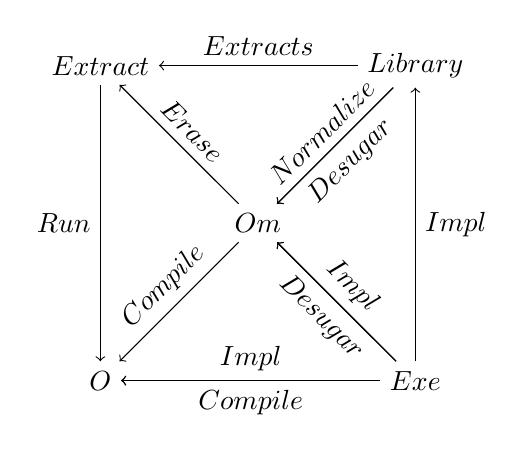
\begin{tikzpicture}
\tikzstyle{every initial by arrow}=[]
    \node (a) at (0,0) {$O$};
    \node (b) at (0,4) {$Extract$};
    \node (c) at (4,0) {$Exe$};
    \node (d) at (4,4) {$Library$};
    \node (e) at (2,2) {$Om$};
    \draw [->] (b) to node [left] {$Run$} (a);
    \draw [->] (c) to node [below] {$Compile$} (a);
    \draw [->] (c) to node [above] {$Impl$} (a);
    \draw [->] (e) to node [above,sloped] {$Compile$} (a);
    \draw [->] (d) to node [above,sloped] {$Normalize$} (e);
    \draw [->] (d) to node [below,sloped] {$Desugar$} (e);
    \draw [->] (d) to node [above] {$Extracts$} (b);
    \draw [->] (c) to node [right] {$Impl$} (d);
    \draw [->] (e) to node [above,sloped] {$Erase$} (b);
    \draw [->] (c) to node [below,sloped] {$Desugar$} (e);
    \draw [->] (c) to node [above,sloped] {$Impl$} (e);
\end{tikzpicture}
\end{center}

\begin{fullwidth}
\hspace{-2cm}
\begin{tabular}{lll}
  $Exe \xrightarrow{Impl} Om$ &---& На прувері пишеться ядро \\
  $Exe \xrightarrow{Impl} O$ &---& На прувері пишеться інтерпретатор \\
  $Exe \xrightarrow{Impl} Exe$ &---& Прувер написаний сам на собі \\
  $Exe \xrightarrow{Impl} Library$ &---& На прувері пишеться базова бібліотека \\
  $Exe \xrightarrow{Desugar} Om$ &---& Сам прувер є розширенням ядра \\
  $Library \xrightarrow{Desugar} Om$ &---& Базова бібліотека конвертується в код ядра \\
  $Library \xrightarrow{Normalize} Om$ &---& Повна нормалізація базової бібліотеки \\
  $Om \xrightarrow{Erase} Extract$ &---& Видаляється інформація про типи, детипізація \\
  $Extract \xrightarrow{Run} O$ &---& Запуск на інтерпритаторі \\
\end{tabular}
\end{fullwidth}


\addtocontents{toc}{\protect\newpage}

\chapter{СЕРЕДОВИЩЕ ВИКОНАННЯ \\ТА МОВИ ПРОГРАМУВАННЯ}

Другий розділ описує розвиток концептуальної моделі системи доведення теорем
як послідовності мов програмування, кожна наступна з яких, складніша за попередню,
має свою операційну семантику, та наслідує усі властивості попередніх мов послідовності.

\section{Пререквізити}

Для розповіді про систему доведення теорем, як систему мов програмування
будемо використовувати теорію категорії та теорію інтуктивниї
типів для специфікації синтаксисів мов програмування. Уся необхідна формальна теорія:
лямбда числення, теорії індуктивних типів, вищі рівності для гомотопічної системи,
тощо, містяться в розділі 3. Формальна теорія категорії міститься у розділі 4.
Слід зауважити, що ця формалізація проводить на основі гомотопічної
мови програмування побудованої в даному розділі 2.

\section*{Середовища виконання та інтерпретатори}

З точки зору класу систем, нас цікавлять всі системи з залежними типами,
як основа теорії типів Мартіна-Льофа та гомотопічної теорії типів. Однак
якщо терм лежить у просторі функцій та не містить елемнтів Path-типу та
вищих гомотопічних типів, такий терм може бути виконаний
на віртуальній машині $O_{CPS}$ або екстрагований у одну з мов лямбда кубу:

$$
O_{CPS}\ ,\ System\ {F}\ ,\ System\ {F_\omega}\ ,\ O_{PTS}
$$

Далі буде йтися тільки про формальні інтерпретатори,
так як вони є найбільш компакними формами мов для верифікації.

\begin{definition} (Інтерпретатор). Інтерпретатор визначається
своїм трьома конструкторами: номер змінної (індекс де Брейна),
лямбда функція та її апплікація:
\begin{lstlisting}
data CPS = var (x: nat)
         | lam (l: nat) (d: cps)
         | app (f a: cps)
\end{lstlisting}
Мовою інтерпретаторів є нетипизоване лямбда числення, однак в залежності
від складності інтерпретатора це дерево може виглядати по-різному.
\end{definition}

В цьому розділі ми побудуємо надшвидку імплементацію інтерпретатора,
яка цілком разом зі своїми програмами розміщується в кеш-памяті
першого рівня процесора, та здатна до AVX векторизацій засобами мови Rust.
Як промислова опція, підтримується також екстракт
в байт-код інтерпретатора BEAM віртуальної машини Erlang.

\section*{Формальні мови програмування}

Тут йдеться про мови програмування придатні для доведення теорем,
та їх таксономію від найелементарніших (чистої системи з одним типом $\Pi$) до
найпотужніших гомотопічних систем. Одна така гомотопічна система є кінцевим завданням
цього розділу --- побудова моделі гомотопічного верифікатора.
В процесі його побудови в цьому розділі ми розглянемо під
мікроскопом складові частини його нижчих мовних рівнів.

Застосуємо категорну семантику для мов програмування і будемо розглядати
мови програмування як моноїдальні мовні категорі, об'єкти яких є просторами
усіх програм цих мов програмування, а морфізми --- правила верифікації та компіляції цих мов.
Морфізми між мовними категоріями в категорї мов програмування --- це
функтори підвищення та пониження складності мови, подібно до того як діють
морфізми в контекстуальних категоріях. Морфізм деконструює або конструює за
допомогою Either-типу або $\Sigma$-типу індуктивний тип мови програмування.

\begin{definition} (Мова програмування).
Мова програмування --- це категорія, єдиний об’єкт якої це
Maybe-типи синтаксичних дерев мов програмування, а морфізми --- це стрілки,
які містять правила виводу, типизації, нормалізації, екстактів, тощо.
Морфізми мовних категорій --- правила виводу, компіляції, верифікації.
Приклади синтаксичних дерев: $O_\Pi$, $O_\Sigma$, $O_=$.
Приклади: $O_{PTS}$, $O_{MLTT$, $O_{HTS}$.
\end{definition}

\begin{definition} (Синтаксичне дерево).
Об'єкти мовних категорій --- Maybe-типи синтаксичних дерев мов програмування.
Синтаксичне дерево --- це індуктивний тип, контруктори якого відповідають
одному з 5 правил в теорії типів, як правило використовуються три правила:
правило формації, інтро-правила та елімінатор.

\begin{definition} (Типи синтаксичних дерев).
Синтаксичні дерева мови програмування в свою чергу діляться на 5 типів:
i) $O_\Pi$ або $O_{PTS}$ --- числення конструкцій, $\Pi$-тип або чиста система;
ii) $O_\Sigma$ --- мова $\Sigma$-типа для вбудовування в ядро;
ii) $O_{=}$ --- мова для Id-типа для вбудовування в ядро;
iv) $O_{*}$ --- числення індуктивних типів (CiC);
v) $O_{I}$ --- гомотопічна мова з вищими індуктивними типами.
\end{definition}

% \newpage
\subsubsection*{Спектр формальних мов}

Мови з залежними типами розкладаються у
спектральну (індексовану натуральними числами $N \rightarrow U$)
послідовність  мов, кожен елемент якої є мовою програмування,
яка не містить синтаксичне дерево вищої мови програмування.
Синтаксичні дерева мов програмування позначаються $O_\Pi$,
$O_\Sigma$, $O_{=}$ , $O_{*}$ , $O_{I}$.

\begin{definition} (Створення мовної категорії).
Мови можна додавати, наприклад $O_{MLTT} = O_{\Pi\Sigma=}$, для побудови якої необхідно
об'єднати у індуктивному типі мови усі індуктивні типи її підмов.
Таким чином функтор діє на декартовому добутку синтаксичних дерев мовних категорій
та має значення в категорій мовних категорій
$O_{MLTT} : O_\Pi \rightarrow O_\Sigma \rightarrow O_= \rightarrow U$.
\end{definition}

Кожне синтаксичне дерево, як правило, містить конструктори
та елімінатори певного одного типу. Але починаючи з $O_{IND}$
складність типів, які додаються до ядра значно зростає.
Таким чином мовні категорії конструються гранулярно з
точністю до включення певного типу в ядро верифікатора.

\begin{definition} (Система мов).
Так, виділяється наступна послідовність мов, та функторів між ними,
де кожна мова-кодомен є складнішою та біль потужною за мову-домен.
Система мов є категорією мовних категорій або категорією мов програмування.
$$
O_{PTS} \rightarrow O_{MLTT} \rightarrow O_{IND} \rightarrow O_{HTS}.
$$
\end{definition}

\newpage

\subsubsection{Чиста система $O_{PTS}$}

Чиста ситема або числення конструкцій або система з одим типом або
система з однією аксіомою, продовжує традиції елементарних пруверів
в стилі першого AUTOMATH та сучасного Morte, Henk.

\begin{definition} (Мовна категорія чистої мови $O_{PTS}$).
$$
O_{PTS} =
\begin{cases}
Ob: \begin{cases}
X: maybe\ PTS \\
target: maybe\ CPS \\
\end{cases} \\
Hom: \begin{cases}
type,norm: X \rightarrow X \\
extract: X \rightarrow target \\
certify: X \rightarrow target = type \circ norm \circ extract
\end{cases}
\end{cases}
$$
\end{definition}

\begin{definition} (Синтаксис мовної категорії $O_{PTS}$).
Чиста мова $O_{PTS}$ містить лише синтаксис одного типу, $\Pi$-типу.
Така теорія називається теорією з одним типом, або з однією аксіомою.
\begin{lstlisting}[mathescape=true]
data PTS = ppure (_: pts PTS)
\end{lstlisting}
\end{definition}

Вона описана в літературі як Calculus of Construction (Кокан),
Pure Type System (Стемп, Фу).

\begin{definition} (Синтаксичне дерево $O_\Pi$).
\begin{lstlisting}[mathescape=true]
data pts (lang: U)
   = star (n: nat)
   | var (x: name) (l: nat)
   | pi (x: name) (l: nat) (f: lang)
   | lambda  (x: name) (l: nat) (f: lang)
   | app (f a: lang)
\end{lstlisting}
\end{definition}

\newpage
\subsubsection{Теорія типів Мартіна-Льофа $O_{MLTT}$}

Мова теорії типів є сучасною основою всіх пруверів з залежними типами,
такими, наприклад, як NuPRL та Agda. Багато так званих $\Pi\Sigma$ пруверів
імплементують $MLTT$ серед таких як:
$\Pi\Sigma$\footnote{\url{https://github.com/zlizta/pisigma-0-2-2}},
$\Pi\forall$\footnote{\url{https://github.com/sweirich/pi-forall}}.

\begin{definition} (Мовна категорія $O_{MLTT}$).
$$
O_{MLTT} =
\begin{cases}
Ob: maybe\ MLTT \\
Hom: \begin{cases}
type,norm: Ob \rightarrow Ob \\
certify: Ob \rightarrow Ob = type \circ norm \\
\end{cases}
\end{cases}
$$
\end{definition}

\begin{definition} (Синтаксис мовної категорії $O_{MLTT}$).
Мова $O_{MLTT}$ включає в себе синтаксиси трьох типів
теорії Мартіна-Льофа: $O_\Pi$, $O_\Sigma$, $O_=$.
\begin{lstlisting}
data MLTT = mpure (_: pts MLTT)
          | msigma (_: exists MLTT)
          | mid (_: identity MLTT)
\end{lstlisting}
\end{definition}

\begin{definition} (Синтаксичне дерево $O_\Sigma$).
Також можна до чистої системи додати $\Sigma$-тип,
піднявши типову систему до мови $O_{MLTT-72}$ або $O_{\Pi\Sigma}$ :
\begin{lstlisting}[mathescape=true]
data exists (lang: U)
   = sigma (n: name) (a b: lang)
   | pair (a b: lang)
   | fst (p: lang)
   | snd (p: lang)
\end{lstlisting}
\end{definition}

\begin{definition} (Синтаксичне дерево $O_=$).
Додавши тип рівності можно підняти систему ще на одну сходинку,
до $O_{MLTT-84}$ або $O_{\Pi\Sigma=}$:
\begin{lstlisting}[mathescape=true]
data identity (lang: U)
   = id (t a b: lang)
   | id_intro (a b: lang)
   | id_elim (a b c d e: lang)
\end{lstlisting}
\end{definition}

\newpage
\subsubsection{Індуктивна мова $O_{IND}$}

\begin{definition} (Мовна категорія $O_{IND}$).
$$
O_{IND} =
\begin{cases}
Ob: \begin{cases}
X: maybe\ IND \\
target: maybe\ CPS \\
\end{cases} \\
Hom: \begin{cases}
type,norm,induction: X \rightarrow X \\
extract: X \rightarrow target \\
certify: X \rightarrow target = type \circ norm \circ induction \circ extract \\
\end{cases}
\end{cases}
$$

Мова індуктивних типів дозволяє безпосередньо кодувати індуктивні типи,
не використовуючи схеми кодування Бома, містить усі попередні мовні синтаксиси:
$O_=$, $O_\Sigma$, $O_\Pi$.

\begin{definition} (Синтаксичне дерево мовної категорії $O_{IND}$).
\begin{lstlisting}
data IND = ipure (_: pts IND)
         | isigma (_: exists IND)
         | iid (_: identity IND)
         | iind (_: ind IND)
\end{lstlisting}

Мова містить наступні допоміжні визначення: i) телескопу,
який містить послідовність елементів мови; ii) розгалуження,
як конструкцій case оператора; iii) імен конструкторів індуктивного типу.

\begin{lstlisting}
data tele (A: U)   = emp | tel (n: name) (b: A) (t: tele A)
data branch (A: U) =        br (n: name) (args: list name) (term: A)
data label (A: U)  =       lab (n: name) (t: tele A)
                         | com (n: name) (t: tele A) (dim: list name)
                               (str: list (prod (prod name bool) A))
\end{lstlisting}

\begin{definition} (Синтаксичне дерево $O_*$).
Правило формації, конструктора та елімінатора визначається синтаксичним деревом $O_*$:
\begin{lstlisting}
data ind (lang: U)
   = data_  (n: name) (t: tele lang) (labels:   list (label lang))
   | case   (n: name) (t: lang)      (branches: list (branch lang))
   | ctor   (n: name)                (args:     list lang)
\end{lstlisting}

\newpage
\subsubsection{Гомотопічна мова $O_{HTS}$}

\begin{definition} (Мовна категорія $O_{HTS}$).
$$
O_{HTS} =
\begin{cases}
Ob: maybe\ HTS \\
Hom: \begin{cases}
type,norm: Ob \rightarrow Ob \\
certify: Ob \rightarrow Ob = type \circ norm \\
\end{cases}
\end{cases}
$$
\end{definition}

Синтаксис гомотопічна система доведення містить усі
попередні мовні синтаксиси: $O_I$, $O_*$, $O_=$ $O_\Sigma$, $O_\Pi$.

\begin{definition} (Синтаксис мовної категорії $O_{HTS}$).
\begin{lstlisting}
data HTS = hpure (_: pts HTS)
         | hsigma (_: exists HTS)
         | hid (_: identity HTS)
         | hind (_: ind HTS)
         | homotopy (_: hts HTS)
\end{lstlisting}
\end{definition}

Гомотопічна типа наслідує $O_{IND}$ але модифіковану з
Path-типом в індуктивних визначеннях, структурою композиції,
анонсує Path-тип (формація, конструктор, та елімінатор)
як лямбда функцію на відрізку, а також склейку типів у всесвіті
та склейку змінних з відповідними елімінаторами. 

\begin{definition} (Синтаксичне дерево $O_I$).
\begin{lstlisting}
data hts (lang: U)
   = path (t a b: lang)
   | plam (n: name) (a: alg) (b: lang)
   | papp (f: name) (a: lang) (p: alg)
   | comp_ (a b: lang)
   | fill_ (a b c: lang)
   | glue_ (a b c: lang)
   | glue_elem (a b: lang)
   | unglue_elem (a b: lang)
\end{lstlisting}
\end{definition}

Таким чином,
$O_{HTS}$ містить два Id-типа, один унаслідований від $O_=$,
а інший який міститься в синтаксичному дереві $O_I$.

\\

Кожна секція цієї глави буде присвячена цим мовним компонентам
системи доведення теорем. В кінці розділу дається повна система, яка включає в себе усі
мови та усі мовні перетворення.

\newpage
\section{Інтерпретатор та середовище виконання}

Мінімаль мова системи $O_{CPS}$ визначається простим
синтаксичним деревом

\begin{lstlisting}
data cps = var (x: nat)
         | lam (l: nat) (d: cps)
         | app (f a: cps)
\end{lstlisting}

Однак, на практиці, застосовують більш складні описи синтаксичних дерев,
зокрема для лінивих обчислень, та розширення синтаксичного дерева спеціальними
командами пов'язаними з середовищем виконання. Програми таких
інтерпретаторів відповідно виконуються у певній пам'яті, яка
використовується як контекст виконання. Кожна така програма крутиться
як одиниця виконання на певному ядрі процесора. Ситема процесів, де
кожен процес є CPS-програмою яку виконує інтерпретатор на певному ядрі.

Мотивація для побудови такого інтерпретатору, який повністю розміщується
разом зі программою в L1 стеку (який лімітований 64КБ) базується на успіху
таких віртуальних машин як LuaJIT, V8, HotSpot, а також векторних мов
програмування типу К та J. Якби ми могли побудувати дійсно швидкий інтерпретатор
який би виконував програми цілком в L1 кеші, байткод та стріми якого були би
вирівняні по словам архітектури, а для векторних обчислень застосовувалися би AVX обчислення,
які, як відомо перемагають по ціні-якості GPU обчислення. Таким чином, такий
інтерпретатор міг би, навіть без спеціалізованої JIT компіляції, скласти
конкуренцію сучасним промисловим інтерпретаторам, таким як Erlang, Python, K, LuaJIT.

Для дослідження цієї гіпотези мною було побудовано еспериментальний інтерпретатор
без байт-коду, але з вирівняним по словам архітерктури стріму команд, які є
безпосередньою машинною презентацією конструкторів індуктивних типів (enum) мови Rust.
Наступні результати були отримані після неотпимізованої версії інтерпретатора
пнри обчисленні факторіала (5) та функції Акермана у точці (3,4).

\begin{lstlisting}
Rust    0
Java    3
PyPy    8
O-CPS   291
Python  537
K       756
Erlang  10699/1806/436/9
LuaJIT  33856
\end{lstlisting}

\begin{lstlisting}
akkerman_k     635 ns/iter (+/- 73)
akkerman_rust  8,968 ns/iter (+/- 322)
\end{lstlisting}

Ключовим викликом тут стали лінійні типи мови Rust, які не дозволяють
звертатися до ссилок, які вже були оброблені, а це впливає на всю
архітектуру тензорного преставлення змінних в мові інтерпретатор $О_{CPS}$,
яка наслідує певним чином мову К.

\subsection{Векторизація засобами мови Rust}

\begin{lstlisting}
objdump ./target/release/o -d | grep mulpd
   223f1: c5 f5 59 0c d3    vmulpd (%rbx,%rdx,8),%ymm1,%ymm1
   223f6: c5 dd 59 64 d3 20 vmulpd 0x20(%rbx,%rdx,8),%ymm4,%ymm4
   22416: c5 f5 59 4c d3 40 vmulpd 0x40(%rbx,%rdx,8),%ymm1,%ymm1
   2241c: c5 dd 59 64 d3 60 vmulpd 0x60(%rbx,%rdx,8),%ymm4,%ymm4
   2264d: c5 f5 59 0c d3    vmulpd (%rbx,%rdx,8),%ymm1,%ymm1
   22652: c5 e5 59 5c d3 20 vmulpd 0x20(%rbx,%rdx,8),%ymm3,%ymm3
\end{lstlisting}

\subsection{Байт-код інтерпретатора}

Синтаксичне дерево, або неформалізований бай-код віртуальної
машини або інтерпретатора $O_{CPS}$ розкладається на два дерева, одне дерево
для управляючих команд інтерпретатора: Defer, Continuation, Start (початок програми),
Return (завершення програми).

\begin{lstlisting}
data Lazy = Defer (otree: NodeId) (a: AST) (cont: Cont)
          | Continuation (otree: NodeId) (a: AST) (cont: Cont)
          | Return (a: AST)
          | Start
\end{lstlisting}

Операції віртуальної машини: умовний оператор, оператор присвоєння, лямбда
функція та аплікація, є відображеннями на конструктори синтаксичного дерева.

\begin{lstlisting}
data Cont = Expressions (ast: AST) Option (vec: Iter AST) (cont: Cont)
          | Assign (ast: AST) (cont: Cont)
          | Cond (c,d: AST) (cont: Cont)
          | Func (a,b,c: AST) (cont: Cont)
          | List (acc: Vec AST) (vec: Iter AST) (i: Nat) (cont: Cont)
          | Call (a: AST) (i: Nat) (cont: Cont)
          | Return
          | Intercore (m: Message) (cont: Cont)
          | Yield (cont: Cont)
\end{lstlisting}


\newpage
\subsection{Синтаксис}

Синтаксис мови $O_{CPS}$ підтримує тензори, та звичайне лямбда числення
з значеннями у тензорах машинних типів даних: i32, i64.

\begin{lstlisting}[mathescape=true]
E: V | A | C
NC: ";" = [] | ";" m:NL = m
FC: ";" = [] | ";" m:FL = m
EC: ";" = [] | ";" m:EL = m
NL: NAME | o:NAME m:NC = Cons o m
FL: E | o:E | m:FC = Cons o m
EL: E | EC  | o:E m:EC = Cons o m
C: N | c:N a:C = Call c a
N: NAME | S | HEX | L | F
L: "(" ")" = [] | "([" c:NL "]" m:FL ")" = Table c m | "(" l:EL ")" = List l
F: "{" "}" = Lambda [] [] [] | "{[" c:NL "]" m:EL "}" = Lambda [] c m
                             | "{" m:EL "}" = Lambda [] [] m
\end{lstlisting}

Після парсера, синтаксичне дерево розкладається по наступним складовим: AST для
тензорів, визначення вищого рівня, Value для машинних слів, Scalar для
конструкцій мови, куд входить зокрема: списки та словники, умовний оператор,
присвоєння, визначення функції та її аплікація, UTF-8 літерал, та оператор
передачі управління в поток планувальника який закріплений за певним ядром CPU.

\begin{lstlisting}
data AST     = Atom (a: Scalar)
             | Vector (a: Vec AST)
\end{lstlisting}

\begin{lstlisting}
data Value   = Nil
             | SymbolInt (a: u16)
             | SequenceInt (a: u16)
             | Number (a: i64)
             | Float (a: f64)
             | VecNumber (Vec i64)
             | VecFloat (Vec f64)
\end{lstlisting}

\begin{lstlisting}
data Scalar  = Nil
             | Any
             | List (a: AST)
             | Dict (a: AST)
             | Call (a b: AST)
             | Assign (a b: AST)
             | Cond (a b c: AST)
             | Lambda (otree: Option NodeId) (a b: AST)
             | Yield (c: Context)
             | Value (v: Value)
             | Name (s: String)
\end{lstlisting}

\newpage
\subsection{Операційна система}

\subsection{Властивості}

\subsubsection{Низьколатентний транспорт InterCore}

Шина InterCore конструюється певним числом SPMC черг, виділених для певного ядра.
Шина сама має топологію зірки між ядрами, та черга MPSC організована
як функція над множиною паблішерів. Кожне ядро має рівно одного паблішера.
Функція обробки шини протоколу InterCore називається poll\_bus та є членом планувальника.
Ви можете думати про InterCore як телепорт між процесорами, так як pull\_bus
викликається після кожної операції Yield в планувальник, і, таким чином,
якщо певному ядру опублікували в його чергу повідомлення, то після наступного Yield
на цьому ядрі буде виконана функція обробки цього повідомлення.

\subsubsection*{\lstinline{pub [ capacity ]}}
Створює новий CAS курсор для паблішінга, тобто для запису.
Повертає глобальних машинний ідентифікатор, має єдиний параметр, розмір черги.
Приклад: p: pub[16].

\subsubsection*{\lstinline{sub [ publisher ]}}
Створює новий CAS курсор для читання певної черги, певного врайтера.
Повертає глобальний машинний ідентифікатор для читання.
Приклад: s: sub[p].

\subsubsection*{\lstinline{spawn [ core ; program ; cursors ]}}
Створює нову програму задачу CPS-інтепреторатора для певного ядра.
Задача може бути або програмою на мові Rust або будь якою програмою через FFI.
Також при створенні задачі задається список курсорів,
які ексклюзивно належатимуть до цієї задачі.
Параметри функції: ядро, текст програми або назва FFI функції,спсисок курсорів.
Приклад: spawn[0;"etc/proc0";(0;1)].

\subsubsection*{\lstinline{snd [ writer ; data ]}}
Посилає певні дані в певний курсор для запису. Повертає Nil якшо всьо ОК.
Приклад: snd[p;42].

\subsubsection*{\lstinline{rcv [ reader ]}}
Повертає прочитані дані з певного курсору.
Якшо даних немає, то передає управління в планувальних за допомогою Yield.
Приклад: rcv[s].

\subsection{Структури ядра}
Ядро є ситемою акторів з двома основними типами акторів:
чергами, які представляють кільцеві буфери та відрізки памяті;
та задачами, які резпрезентують байт-код програм та іх інтерпретацію на процесорі.
Черги бувають двох видів: для публікації, які місять курсори для запису;
та для читання, які містять курсори для читання. Задачі можна імплементувати
як Rust програми, або як $O_{CPS}$ програми.

\subsubsection{Черга для публікації}
\begin{lstlisting}
pub struct Publisher<T> {
    ring: Arc<RingBuffer<T>>,
    next: Cell<Sequence>,
    cursors: UncheckedUnsafeArc<Vec<Cursor>>,
}
\end{lstlisting}

\subsubsection{Черга для читання}
\begin{lstlisting}
pub struct Subscriber<T> {
    ring: Arc<RingBuffer<T>>,
    token: usize,
    next: Cell<Sequence>,
    cursors: UncheckedUnsafeArc<Vec<Cursor>>,
}
\end{lstlisting}

Існує дві спецільні задачі: InterCore задача, написана на Rust,
та запускається на всіх ядрах при запуску системи, а також CPS-інтерпретор
головного термінала системи, цей інтерпретор запускається на BSP ядрі,
поближче до Console та WebSocket IO селекторів.
В процесі життя різні CPS та Rust задачі можуть бути запущені в такій системі,
поєднуючи гнучкість програм інтерпретатора, та низькорівненивих програм написаних на мові Rust.

Окрім черг та задач, в системі присутні також таймери та інші IO задачі,
такі як сервери мережі або сервери доступу до файлів. Також існують
структури які репрезентують ядра та містять палнувальники.
Уся віртуальна машина є сукупністю таких структур-ядер.

\paragraph{}
\subsubsection{Канал}
Канал складається з одного курсору для запису та багатьох курсорів для читання.
Канал предствляє собою компонент зірки шини InterCore.
\begin{lstlisting}
pub struct Channel {
    publisher: Publisher<Message>,
    subscribers: Vec<Subscriber<Message>>,
}
\end{lstlisting}

\subsubsection{Черги ядра}
Память репрезентує усі наявні черги для публікації та читання на ядрі.
Ця інформація передається клонованую кожній задачі планувальника на цьому ядрі.
\begin{lstlisting}
pub struct Memory<'a> {
    publishers: Vec<Publisher<Value<'a>>,
    subscribers: Vec<Subscriber<Value<'a>>>,
}
\end{lstlisting}

\subsubsection{Планувальник}
Планувальник репрезентує ядро процесара,
які розрізняються як BSP-ядра (або 0-ядра, bootstrap)
та AP ядра (інші ядра > 0, application). BSP ядро
тримає на собі Console та WebSocket IO селектори.
Це означає, що BSP ядро дає свій час ядру, у той час як AP процесори не обтяжені
таким навантаженням (io черга в таких планувальниках пуста).
Існує InterCore повідомлення яке додає або видаляє довільні IO селектори
в планувальних для довільних конфігурацій.

\begin{lstlisting}
pub struct Scheduler<'a> {
    pub tasks: Vec<T3<Job<'a>>>,
    pub bus: Channel,
    pub queues: Memory<'a>,
    pub io: IO,
}
\end{lstlisting}

\subsection{Протокол InterCore}

\begin{lstlisting}
pub enum Message {
    Pub(Pub),
    Sub(Sub),
    Print(String),
    Spawn(Spawn),
    AckSub(AckSub),
    AckPub(AckPub),
    AckSpawn(AckSpawn),
    Exec(usize, String),
    Select(String, u16),
    QoS(u8, u8, u8),
    Halt,
    Nop,
}
\end{lstlisting}

\newpage
\section{Чиста система}

IEEE\footnote{IEEE Std 1012-2016  --- V\&V Software verification and validation} standard
and ESA\footnote{ESA PSS-05-10 1-1 1995 -- Guide to software verification and validation} regulatory documents define a number of tools and approaches for verification and validation processes. 
The most advanced techniques involve mathematical languages and notations. 
The age of verified math was started by de Bruin's AUTOMATH prover and Martin-Löf\cite{Lof84}'s type theory. 
Today we have Coq, Agda, Lean, Idris, F* languages which are based on Calculus of Inductive Constructions or CiC\cite{Mohring15}.
The core of CiC is Calculus of Constructions or CoC\cite{Coq88}.
Further development has lead to Lambda Cube\cite{Henk93} and Pure Type Systems by Henk\cite{Erik97} and Morte\footnote{Gabriel Gonzalez. Haskell Morte Library}.
Pure Type Systems are custom languages based on CoC with single Pi-type and possibly other extensions.
Notable extensions are ECC, ECC with Inductive Types\cite{Ore92}, K-rules\cite{Barthe95}.
The main motivation of Pure Type Systems is an easy reasoning about core, strong normalization and trusted external verification due to compact type checkers.
A custom type checker can be implemented to run certified programs retrieved over untrusted channels.
The applications of such minimal cores are 1) Blockchain smart-contract languages, 2) certified applications kernels, 3) payment processing, etc.

\subsection{Генерація сертифікованих програм}
According to Curry-Howard, a correspondence inside Martin-Löf Type Theory\cite{Lof84} proofs or certificates are lambda terms of particular types or specifications.
As both specifications and implementations are done in a typed language with dependent types we can extract target implementation of a certified program just in any programming language.
These languages could be so primitive as untyped lambda calculus and are usually implemented as untyped interpreters (JavaScript, Erlang, PyPy, LuaJIT, K).
The most advanced approach is code generation to higher-level languages such as C++ and Rust (which is already language with trusted features on memory, variable accessing, linear types, etc.).
In this work, we present a simple code extraction to Erlang programming language as a target interpreter.
However, we have also worked on C++ and Rust targets as well.

{\bf Om} as a programming language has a core type system, the {\bf PTS$^{\infty}$} --- the pure type system with the infinite number of universes.
This type system represents the core of the language.
Higher languages form a set of front-ends to this core.
 Here is example of possible languages:
1) Language for inductive reasoning, based on CiC with extensions;
2) Homotopy Core with interval [0,1] for proving J and funExt;
3) Stream Calculus for deep stream fusion (Futhark);
3) Pi-calculus for linear types, coinductive reasoning and runtime modeling (Erlang, Ling, Rust).
These languages desugar to {\bf PTS$^{\infty}$} as an intermediate language before extracting to target language\footnote{Note that extracting from [0,1] Homotopy Core is an open problem}.

Not all terms from higher languages could be desugared to PTS.
As was shown by Geuvers\cite{Geuvers01} we cannot build induction principle inside PTS, we need a fixpoint extension to PTS.
And also we cannot build the J and funExt terms.
But still PTS is very powerful, it's compatible with System F libraries.
The properties of that libraries could be proven in higher languages with Induction and/or [0,1] Homotopy Core.
Then runtime part could be refined to PTS, extracted to target and run in an environment.

We see two levels of extensions to PTS core: 1) Inductive Types support; 2) Homotopy Core with [0,1] and its eliminators.
We will touch a bit this topic in the last section of this document.

{\bf PTS синтаксиси}. Мінімальне ядро з однією аксіомою
сприймає декілька лямбда ситаксисів.
Перший синтаксис сумісний з системою програмування
$morte$\footnote{http://github.com/Gabriel439/Haskell-Morte-Library}, та походить від неї.
Інший синтаксис сумісний з синтаксисом $cubical$\footnote{http://github.com/mortberg/cubicaltt}.
Планувалося також підтримати синтаксис $caramel$\footnote{https://github.com/MaiaVictor/caramel}.

\begin{table}[h]
\begin{center}
\caption{List of languages, tried as verification targets}
\label{tab:a}
\tabcolsep7pt\begin{tabular}{lcccc}
\hline
{\bf Target} & {\bf Class} & {\bf Intermediate} & {\bf Theory}\\
\hline
C++        & compiler/native      & HNC & System F\\
Rust       & compiler/native      & HNC & System F\\
JVM        & interpreter/native   & Java    & F-sub\footnote{System F wit bounded quantification}\\
JVM        & interpreter/native   & Scala   & System F-omega\\
GHC Core   & compiler/native      & Haskell & System D\\
GHC Core   & compiler/native      & Morte   & CoC\\
Haskell    & compiler/native      & Coq     & CiC\\
OCaml      & compiler/native      & Coq     & CiC\\
{\bf BEAM} & {\bf interpreter} & {\bf Om}   & {\bf PTS$^\infty$} \\
O          & interpreter          & Om  & PTS$^\infty$ \\
K          & interpreter          & Q   & Applicative \\
PyPy       & interpreter/native   & N/A & ULC \\
LuaJIT     & interpreter/native   & N/A & ULC \\
JavaScript & interpreter/native & PureScript & System F\\
\hline
\end{tabular}
\end{center}
\end{table}

Мова програмування Ом -- це мова з залежними типами, яка є розширенням
числення конструкцій (Calculus of Constructions, CoC) Тері Кокуанда. Саме з числення
конструкцій починається сучасна обчислювальна математика. В додаток до CoC,
наша мова Ом має предикативну ієрархію індексованих всесвітів. В цій мові немає
аксіоми рекурсії для безпосереднього визначення рекурсивних типів. Однак в цій мові
вцілому, рекурсивні дерева та корекурсія може бути визначена, або як кажуть, закодована.
Така система аксіом називається системою з однією аксіомою (або чистою системою), тому що в ній
існує тільки Пі-тип, а для кожного типу в теорії типів Мартіна Льофа існує п'ять
конструкцій: формація, інтро, елімінатор, бета та ета правила.

Усі терми підчиняються системі аксіом $Axioms$ всередині послідовності всесвітів $Sorts$
та складність залежного терму відповідає максимальній складності домена та кодомена (правила $Rules$).
Таким чином визначається простір всесвітів, та його конфігурація може бути записана
згідно нотації Барендрехта для систем з чистими типами:

$$
\begin{cases}
    Sorts = U.\{i\},\ i : Nat\\
    Axioms = U.\{i\} : U.\{inc\ i\}\\
    Rules = U.\{i\} \leadsto U.\{j\} : U.\{max\ i\ j\}\\
\end{cases}
$$

\paragraph{}
An intermediate Om language is based on Henk\cite{henk} languages described first
by Erik Meijer and Simon Peyton Jones in 1997. Leter on in 2015 Morte impementation
of Henk design appeared in Haskell, using Boem-Berrarducci encoding of non-recursive lambda terms.
It is based only on one type constructor $\Pi$, its special case $\lambda$ and theirs eliminators:
$apply$ and $curry$, infinity number of universes,
and one computation rule called $\beta$-reduction.
The design of Om language resemble Henk and Morte both
design and implementation. This language indended to be small, concise, easy provable
and able to produce verifiable peace of code that can be distributed over the networks,
compiled at target with safe trusted linkage.

\newpage
\subsection{Синтаксис}
Om syntax is compatible with $\lambda C$ Coquand's Calculus of Constructions presented
in Morte and Henk languages. However it has extension in a part of specifying
universe index as a {\bf Nat} number.

\vspace{0.5cm}
\begin{lstlisting}[mathescape=true]
    <> := #option
     I := #identifier
     U := * < #number >
     O := U
        | I | ( O ) | O O | O $\rightarrow$ O
        | $\lambda$ ( I : O ) $\rightarrow$ O
        | $\forall$ ( I : O ) $\rightarrow$ O
\end{lstlisting}

Еквівалентне визначення як ініціальний об'єкт категорій $O_{PTS}$ або $O_\Pi$
який може вмістити цей синтаксис містить всі правила виводу
внутрішньої мови категорії.

\begin{lstlisting}[mathescape=true]
data pts (lang: U)
   = star             (n: nat)
   | var    (x: name) (l: nat)
   | pi     (x: name) (l: nat) (d c: lang)
   | lambda (x: name) (l: nat) (d c: lang)
   | app                       (f a: lang)
\end{lstlisting}


\subsection{Всесвіти}

The OM language is a higher-order dependently typed lambda calculus,
an extension of Coquand's Calculus of Constructions
with the predicative/impredicative hierarchy of indexed universes.
This extension is motivated avoiding paradoxes in dependent theory.
Also there is no fixpoint axiom needed for the definition
of infinity term dependance.

\begin{lstlisting}[mathescape=true]
    $U_0$ : $U_1$ : $U_2$ : $U_3$ : ...

    $U_0$ --- propositions
    $U_1$ --- values and sets
    $U_2$ --- types
    $U_3$ --- sorts
\end{lstlisting}

\begin{equation}
\tag{S}
\dfrac
{o : Nat}
{U_o}
\end{equation}

\newpage
\subsection*{Предикативні всесвіти}

All terms obey the A ranking inside the sequence of S universes,
and the complexity R of the dependent term is equal to a maximum of
the term's complexity and its dependency.
The universes system is completely described by the following
PTS notation (due to Barendregt):

Note that predicative universes are incompatible with Church lambda term encoding.
You can switch predicative vs impredicative uninverses by typecheker parameter.

\[
\tag{$A_1$}
\dfrac{i: Nat, j: Nat, i < j}{U_i : U_j}
\]

\[
\tag{$R_1$}
\dfrac{i : Nat, j : Nat}{U_i \rightarrow U_j : U_{max(i,j)} }
\]

\subsection*{Імпредикативні всесвіти}
Propositional contractible bottom space is the only
available extension to predicative hierarchy that not leads to inconsistency.
However there is another option to have infinite
impredicative hierarchy.

\begin{equation}
\tag{$A_2$}
\dfrac
{i: Nat}
{U_i : U_{i+1}}
\end{equation}

\begin{equation}
\tag{$R_2$}
\dfrac
{i : Nat,\ \ \ \ j : Nat}
{U_i \rightarrow U_{j} : U_{j}}
\end{equation}

\subsection{Контексти}

The contexts model a dictionary with variables for type checker.
It can be typed as the list of pairs or {\bf List\ Sigma}.
The elimination rule is not given here as in our implementation the whole dictionary is destroyed after type checking.

\begin{equation}
\tag{Ctx-formation}
\dfrac
{}
{\Gamma : Ctx}
\end{equation}

\begin{equation}
\tag{Ctx-intro$_1$}
\dfrac
{\Gamma : Ctx}
{\emptyset : \Gamma}
\end{equation}

\begin{equation}
\tag{Ctx-intro$_2$}
\dfrac
{A : U_i,\ \ \ \ x : A,\ \ \ \ \Gamma : Ctx}
{(x : A)\ \vdash\ \Gamma : Ctx}
\end{equation}

\newpage
\subsection{Операційна семантика}

This language is called one axiom language (or pure) as eliminator
and introduction rules inferred from type formation rule.
The only computation rule of Pi type is called beta-reduction.
Computational rules of language are called operational semantics
and establish equality of substitution and lambda application.
Operational semantics in that way defines the rewrite rules of computations.

\begin{equation}
\tag{$\Pi$-formation}
\dfrac
{A:U_i\ ,\ x:A \vdash B : U_j}
{\Pi\ (x:A) \rightarrow B : U_{p(i,j)}}
\end{equation}

\begin{equation}
\tag{$\lambda$-intro}
\dfrac
{x:A \vdash b : B}
{\lambda\ (x:A) \rightarrow b : \Pi\ (x: A) \rightarrow B }
\end{equation}

\begin{equation}
\tag{$App$-elimination}
\dfrac
{f: (\Pi\ (x:A) \rightarrow B)\ \ \ a: A}
{f\ a : B\ [a/x]}
\end{equation}

\begin{equation}
\tag{$\beta$-computation}
\dfrac
{x:A \vdash b: B\ \ \ a:A}
{(\lambda\ (x:A) \rightarrow b)\ a = b\ [a/x] : B\ [a/x]}
\end{equation}

\begin{equation}
\tag{subst}
\dfrac
{\pi_1 : A\ \ \ \ u:A \vdash \pi_2 : B}
{[\pi_1/u]\ \pi_2 : B}
\end{equation}

The theorems (specification) of PTS could be embedded in itself and used as
Logical Framework for the Pi type. Here is the example in the higher language.

\begin{lstlisting}[mathescape=true]
PTS (A: U): U
  = (Pi_Former: (A -> U) -> U)
  * (Pi_Intro: (B: A -> U) (a: A) -> B a -> (A -> B a))
  * (Pi_Elim: (B: A -> U) (a: A) -> (A -> B a) -> B a)
  * (Pi_Comp1: (B: A -> U) (a: A) (f: A -> B a) ->
    Path (B a) (Pi_Elim B a (Pi_Intro B a (f a))) (f a))
  * (Pi_Comp2: (B: A -> U) (a: A) (f: A -> B a) ->
    Path (A -> B a) f (\(x:A) -> f x))
\end{lstlisting}

The proofs intentionally left blank, as it proofs could be taken from various sources \cite{Henk93}.
The equalities of computational semantics presented here as {\bf Path} types in the higher language.
The {\bf Om} language is the extention of the {\bf PTS$^\infty$} with the remote AST node which means remote file loading from trusted storage, anyway this will be checked by the type checker.
We deny recursion over the remote node.
We also add an index to var for simplified de Bruijn indexes, we allow overlapped names with tags, incremented on each new occurrence.
Our typechecker differs from cannonical example of Coquand\cite{Coq96}. 
We based our typechecker on variable {\bf Substitution}, variable {\bf Shifting}, term {\bf Normalization}, definitional {\bf Equality} anf {\bf Type Checker} itself.


\subsection{Перевірка типів}

For sure in a pure system, we should be careful with {\bf :remote} AST node.
Remote AST nodes like {\bf \#List/Cons or \#List/map} are remote links to files.
So using trick one should desire circular dependency over {\bf :remote}.

\begin{lstlisting}[mathescape=true]
type (:star,N)   D $\rightarrow$ (:star,N+1)
   (:var,N,I)    D $\rightarrow$ :true = proplists:is_defined N B, om:keyget N D I
   (:remote,N)   D $\rightarrow$ om:cache (type N D)
   (:pi,N,0,I,O) D $\rightarrow$ (:star,h(star(type I D)),star(type O [(N,norm I)|D]))
   (:fn,N,0,I,O) D $\rightarrow$ let star (type I D), NI = norm I
                       in (:pi,N,0,NI,type(O,[(N,NI)|D]))
   (:app,F,A)    D $\rightarrow$ let T = type(F,D),
                          (:pi,N,0,I,O) = T, :true = eq I (type A D)
                       in norm (subst O N A)
\end{lstlisting}

\subsection{Індекси де Брейна}

Shift renames var N in B. Renaming means adding 1 to the nat component of variable.

\begin{lstlisting}[mathescape=true]
  sh (:star,X)       N P $\rightarrow$ (:star,X)
     (:var,N,I)      N P $\rightarrow$ (:var,N,I+1) when I >= P
                         $\rightarrow$ (:var,N,I)
     (:remote,X)     N P $\rightarrow$ (:remote,X)
     (:pi,N,0,I,O)   N P $\rightarrow$ (:pi,N,0,sh I N P,sh O N P+1)
     (:fn,N,0,I,O)   N P $\rightarrow$ (:fn,N,0,sh I N P,sh O N P+1)
     (:app,L,R)      N P $\rightarrow$ (:app,L,R)
\end{lstlisting}

\subsection{Підстановка, нормалізація, рівність}
Substitution replaces variable occurance in terms.

\begin{lstlisting}[mathescape=true]
 sub (:star,X)     N V L $\rightarrow$ (:star,X)
     (:var,N,L)    N V L $\rightarrow$ V
     (:var,N,I)    N V L $\rightarrow$ (:var,N,I-1) when I > L
     (:remote,X)   N V L $\rightarrow$ (:remote,X)
     (:pi,N,0,I,O) N V L $\rightarrow$ (:pi,N,0,sub I N V L,sub O N (sh V N 0) L+1)
     (:pi,F,X,I,O) N V L $\rightarrow$ (:pi,F,X,sub I N V L,sub O N (sh V F 0) L)
     (:fn,N,0,I,O) N V L $\rightarrow$ (:fn,N,0,sub I N V L,sub O N (sh V N 0) L+1)
     (:fn,F,X,I,O) N V L $\rightarrow$ (:fn,F,X,sub I N V L,sub O N (sh V F 0) L)
     (:app,F,A)    N V L $\rightarrow$ (:app,   sub F N V L,sub A N V L)
\end{lstlisting}

Normalization performs substitutions on applications to functions (beta-reduction)
by recursive entrance over the lambda and pi nodes.

\begin{lstlisting}[mathescape=true]
norm (:star,X)     $\rightarrow$ (:star,X)
     (:var,X)      $\rightarrow$ (:var,X)
     (:remote,N)   $\rightarrow$ cache (norm N [])
     (:pi,N,0,I,O) $\rightarrow$ (:pi,N,0,norm I,norm O)
     (:fn,N,0,I,O) $\rightarrow$ (:fn,N,0,norm I,norm O)
     (:app,F,A)    $\rightarrow$ case norm F of
                         (:fn,N,0,I,O) $\rightarrow$ norm (subst O N A)
                                    NF $\rightarrow$ (:app,NF,norm A) end
\end{lstlisting}

Definitional Equality simply checks the equality of Erlang terms.

\begin{lstlisting}[mathescape=true]
  eq (:star,N)        (:star,N)        $\rightarrow$ true
     (:var,N,I)       (:var,(N,I))     $\rightarrow$ true
     (:remote,N)      (:remote,N)      $\rightarrow$ true
     (:pi,N1,0,I1,O1) (:pi,N2,0,I2,O2) $\rightarrow$
          let :true = eq I1 I2
           in eq O1 (subst (shift O2 N1 0) N2 (:var,N1,0) 0)
     (:fn,N1,0,I1,O1) (:fn,N2,0,I2,O2) $\rightarrow$
          let :true = eq I1 I2
           in eq O1 (subst (shift O2 N1 0) N2 (:var,N1,0) 0)
     (:app,F1,A1)       (:app,F2,A2)   $\rightarrow$ let :true = eq F1 F2 in eq A1 A2
     (A,B)                             $\rightarrow$ (:error,(:eq,A,B))
\end{lstlisting}

\subsection{Використання мови}
Here we will show some examples of {\bf Om} language usage.
In this section, we will show two examples.
One is lifting PTS system to MLTT system by defining {\bf Sigma} and {\bf Equ} types using only {\bf Pi} type.
We will use Bohm inductive dependent encoding\cite{Bohm85}.
The second is to show how to write real world programs in {\bf Om} that performs input/output operations within Erlang environment.
We show both recursive (finite, routine) and corecursive (infinite, coroutine, process) effects.

\begin{lstlisting}
$ ./om help me
[{a,[expr],"to parse. Returns {_,_} or {error,_}."},
 {type,[term],"typechecks and returns type."},
 {erase,[term],"to untyped term. Returns {_,_}."},
 {norm,[term],"normalize term. Returns term's normal form."},
 {file,[name],"load file as binary."},
 {str,[binary],"lexical tokenizer."},
 {parse,[tokens],"parse given tokens into {_,_} term."},
 {fst,[{x,y}],"returns first element of a pair."},
 {snd,[{x,y}],"returns second element of a pair."},
 {debug,[bool],"enable/disable debug output."},
 {mode,[name],"select metaverse folder."},
 {modes,[],"list all metaverses."}]

$ ./om print fst erase norm a "#List/Cons"
   \ Head
-> \ Tail
-> \ Cons
-> \ Nil
-> Cons Head (Tail Cons Nil)
ok
\end{lstlisting}

\subsection{Екстракти}

This works expect to compile to limited target platforms. For now Erlang, Haskell and LLVM is awaiting.
Erlang version is expected to be useful both on LING and BEAM Erlang virtual machines.

\subsubsection{Інтерпретатори}

From a practical point of view, we develop Erlang with Dependent Types.
Thus we carefully integrate with Erlang platform by generating Erlang
AST and trying to be compatible with Erlang kernel through mapping of
inductive types to underlying Erlang primitives such as process,
receive, and spawn. Erlang extraction is sponsored and supported
by Synrc Research Center. Extraction in other languages could also be easily implemented.

\subsubsection{LLVM}

Another branch of research is dedicated to evaluation of LLVM lambda generation. It could be direct MIR or LLVM generation, or we could generate Rust/C++ code that could be passed to LLVM optimizer. If you are interested in LLVM target, please take a look at github.com/nponeccop/HNC.

\subsubsection{FPGA}

We are very interested in compilation to FPGA. As was shown with interaction nets it is possible to compact packaging of inductive construction in silicon, giving back the inner language of space to the natural encoding. If you are interested in moving this project forward and have a vision how to do it please drop us a line in gitter.im/groupoid/exe chat.

\newpage
\section{Індуктивна система}

{\bf Індуктивні синтаксиси}. Індуктивні синтаксиси та кодування можуть підтримуватися за допомогою системи модулів.
Кожна система модулів може самостійно (у вигляді ефектів), або за допомогою лямбда кодувань
попередньої мови PTS рівня, зберігати та оперувати індуктивними типами даних.

\subsection{Синтаксис}

Індуктивні синтаксиси будуються на телескопах Диб'єра,
конструкторах сум, та їх елімінаторах.

\begin{lstlisting}
data tele (A: U)   = emp | tel (n: name) (b: A) (t: tele A)
data branch (A: U) =        br (n: name) (args: list name) (term: A)
data label (A: U)  =       lab (n: name) (t: tele A)
                         | com (n: name) (t: tele A) (dim: list name)
                               (str: list (prod (prod name bool) A))
\end{lstlisting}

\begin{lstlisting}
data ind (lang: U)
   = data_  (n: name) (t: tele lang) (labels:   list (label lang))
   | case   (n: name) (t: lang)      (branches: list (branch lang))
   | ctor   (n: name)                (args:     list lang)
\end{lstlisting}

% \newpage
  \subsection{Поліноміальні функтори}

  \paragraph{}
  There are two types of recursion: one is least fixed point (as $F_A\ X = 1 + A\times X$
  or $F_A\ X = A + X\times X$), in other words the recursion with a base (terminated with a bounded value),
  lists and trees are examples of such recursive structures (so we call induction recursive sums);
  and the second is greatest fixed point or recursion withour a base (as $F_A\ X = A\times X $) ---
  such kind of recursion on infinite lists (codata, streams, coinductive types) we can call recursive products.\\
  Least fixed point trees are called well-founded trees and encode polynomial functors.

  \paragraph{}
  Natural Numbers: $\mu\ X \rightarrow 1 + X$\\
  List A: $\mu\ X \rightarrow 1 + A \times X$\\
  Lambda calculus: $\mu\ X \rightarrow 1 + X \times X + X$\\
  Stream: $\nu\ X \rightarrow A \times X$\\
  Potentialy Infinite List A: $\nu\ X \rightarrow 1 + A \times X$\\
  Finite Tree: $\mu\ X \rightarrow \mu\ Y \rightarrow 1 + X \times Y = \mu\ X = List\ X$\\

  \paragraph{}
  As we know there are several ways to appear for variable in recursive algebraic type.
  Least fixpoint are known as an recursive expressions that have a base of recursion
  Both recursive and corecursive datatypes could be encoded using Boem-Berarducci encoding
  as an non-recursive definitions of folds that include in indentity signature all the
  constructor components of (co)inductive type.

\subsection{Кодування Бома}
The data type of lists over a given set A can be represented as the initial algebra
$(\mu L_A, in)$ of the functor $L_A(X) = 1 + (A \times X)$. Denote $\mu L_A = List(A)$.
The constructor functions $nil: 1 \rightarrow List(A)$ and
$cons: A \times List(A) \rightarrow List(A)$ are defined by
$nil = in \circ inl$ and $cons = in \circ inr$, so $in = [nil,cons]$.
Given any two functions $c: 1 \rightarrow C$ and $h: A \times C \rightarrow C$,
the catamorphism $f = \llparenthesis [c,h] \rrparenthesis : List(A) \rightarrow C$
is the unique solution of the equation system:
$$
\begin{cases}
  f \circ nil  = c \\
  f \circ cons = h \circ (id \times f)
\end{cases}
$$
where $f = foldr(c,h)$. Having this the initial algebra is presented with functor
$\mu (1 + A \times X)$ and morphisms sum $[1 \rightarrow List(A), A \times List(A) \rightarrow List(A)]$
as catamorphism. Using this encdoding the base library of List will have following form:
$$
\begin{cases}
 foldr = \llparenthesis [ f \circ nil , h] \rrparenthesis, f \circ cons = h \circ (id \times f)\\
 len = \llparenthesis [ zero, \lambda\ a\ n \rightarrow succ\ n ] \rrparenthesis \\
 (++) = \lambda\ xs\ ys \rightarrow \llparenthesis [ \lambda (x) \rightarrow ys, cons ] \rrparenthesis (xs) \\
 map = \lambda\ f \rightarrow \llparenthesis [ nil, cons \circ (f \times id)] \rrparenthesis
\end{cases}
$$
\begin{lstlisting}[mathescape=true]
             data list: (A: *) $\rightarrow$ * :=
                  (nil: list A)
                  (cons: A $\rightarrow$ list A $\rightarrow$ list A)
\end{lstlisting}
$$
\begin{cases}
list = \lambda\ ctor \rightarrow \lambda\ cons \rightarrow \lambda\ nil \rightarrow ctor\\
cons = \lambda\ x\ \rightarrow \lambda\ xs \rightarrow \lambda\ list \rightarrow \lambda\ cons \rightarrow\ \lambda\ nil \rightarrow cons\ x\ (xs\ list\ cons\ nil)\\
nil = \lambda\ list \rightarrow \lambda\ cons \rightarrow \lambda\ nil \rightarrow nil\\
\end{cases}
$$
\begin{lstlisting}[mathescape=true]
           record lists: (A B: *) :=
                  (len: list A $\rightarrow$ integer)
                  ((++): list A $\rightarrow$ list A $\rightarrow$ list A)
                  (map: (A $\rightarrow$ B) $\rightarrow$ (list A $\rightarrow$ list B))
                  (filter: (A $\rightarrow$ bool) $\rightarrow$ (list A $\rightarrow$ list A))
\end{lstlisting}
$$
\begin{cases}
len = foldr\ (\lambda\ x\ n \rightarrow succ\ n)\ 0\\
(++) = \lambda\ ys \rightarrow foldr\ cons\ ys\\
map = \lambda\ f \rightarrow foldr\ (\lambda x\ xs \rightarrow cons\ (f\ x)\ xs)\ nil\\
filter = \lambda\ p \rightarrow foldr\ (\lambda x\ xs \rightarrow if\ p\ x\ then\ cons\ x\ xs\ else\ xs)\ nil\\
foldl = \lambda\ f\ v\ xs = foldr\ (\lambda\ xg\rightarrow\ (\lambda \rightarrow g\ (f\ a\ x)))\ id\ xs\ v\\
\end{cases}
$$

\newpage
\section{Гомотопічна система}

\subsection{Синтаксис}


\begin{lstlisting}[mathescape=true]
   sys := [ sides ]          side := (id=0)$\rightarrow$exp+(id=1)$\rightarrow$exp
  form := form\/f1+f1+f2    sides := #empty+cos+side
   cos := side,side+side,cos  mod := ${\bf module}$ id ${\bf where}$ imps dec
    f1 := f1/\f2               f2 := -f2+id+0+1
   imp := ${\bf import}$ id                 brs := #empty+cobrs
   app := exp exp             tel := #empty+cotel
  imps := #list imp         cotel := (exp:exp) tel
    id := #list #nat          dec := #empty+codec
    u2 := ${\bf glue}$+${\bf unglue}$+${\bf Glue}$                   u1 := ${\bf fill}$+${\bf comp}$
   ids := #list id             br := ids$\rightarrow$exp+ids@ids$\rightarrow$exp
 codec := def dec
 cobrs := | br brs
   sum := #empty+id tel+id tel|sum+id tel<ids>sys   
   def := ${\bf data}$ id tel=sum+id tel:exp=exp+id tel:exp ${\bf where}$ def
   exp := cotel*exp+cotel$\rightarrow$exp+exp$\rightarrow$exp+(exp)+id
          (exp,exp)+\cotele$\rightarrow$exp+${\bf split}$ cobrs+exp${\bf.1}$+exp${\bf.2}$+
          $\langle$ids$\rangle$exp+exp@form+app+u2 exp exp sys+u1 exp sys
\end{lstlisting}

Here := (definition), + (disjoint sum), \#empty, \#nat, \#list are parts of BNF language and
$\rvert$, :, *, $\langle$, $\rangle$, (, ), =, $\backslash$, /, -, $\rightarrow$, 0, 1, @, [, ],
$\mathbf{module}$, $\mathbf{import}$,
$\mathbf{data}$, $\mathbf{split}$, $\mathbf{where}$, $\mathbf{comp}$, $\mathbf{fill}$,
$\mathbf{Glue}$, $\mathbf{glue}$, $\mathbf{unglue}$,
$\mathbf{.1}$, $\mathbf{.2}$,
 and $,$ are terminals of type checker language. This language includes
inductive types, higher inductive types and gluening operations needed for
both, the constructive homotopy type theory and univalence. All these concepts as a part of the languages
will be described in the upcoming Issues II---V.

Система не повинна бути обмежена мовами та синтаксисами, ми покажемо як приклад,
підтримку гомотопічної мови з інтервалом [0,1] сумісної з $cubical$ та з пітримкою індуктивних
синтаксисів та кодувань попереднього рівня.

\begin{lstlisting}[mathescape=true]
data alg
   = zero
   | one
   | max (a b: alg)
   | min (a b: alg)

data hts
   = path (t a b: lang)
   | plam (n: name) (a: alg) (b: lang)
   | papp (f: name) (a: lang) (p: alg)
   | comp_ (a b: lang)
   | fill_ (a b c: lang)
   | glue_ (a b c: lang)
   | glue_elem (a b: lang)
   | unglue_elem (a b: lang)
\end{lstlisting}

\section{Гомотопічна базова бібліотека системи доведення}

Як апогей, система HTS є фінальною категорією,
куди сходяться всі стрілки категорії мов. Кожна мова та її категорія
мають певний набір стрілок ендоморфізмів, які обчислюють, верифікують,
нормалізують, оптимізують програми своїх мов.
Стрілки виду $e_i: O_{n+1} \rightarrow O_n$ є екстракторами, які понижають систему типів,
при чому $O_{CPS} = O_0$.

Базова бібліотека мови Ерланг в яку проводиться основний
естракт йде з дистрибутивом Erlang/OTP. Базова бібліотека
$O_{PTS}$ наведена в репозиторії Github\footnote{\url{https://github.com/groupoid/om}}.
Гомотопічна базова бібліотека відповідає термінальній мові $O_{CCHM}$, та теж відкрита
на Github\footnote{\url{https://github.com/groupoid/infinity}}.
Останні два розділи присвячені математичному моделюванню математики на цій мові.

\subsection{Основа}

Перша частина гомотопічної базової бібліотеки --- це основи гомотопічної теорії типів,
з основними визначеннями та теоремами.

\subsection{Математика}

Друга частина гомотопічної базової бібліотеки --- це формалізація математики, як
приклад використання розробленої концепцтуальної моделі системи доведення теорем.

%\section{Числення процесів BPE}

%\section{Числення протоколів N2O}


\newpage
\chapter{Інтерпретатор}

\newpage
\chapter{Базова бібліотека}

\newpage
\chapter{Система доведення теорем}

\newpage

\begin{fullwidth}[width=\linewidth+4cm]
\begin{thebibliography}{99}

%\subsection*{Category Theory}
\bibitem{maclane}    S.MacLane \textit{Categories for the Working Mathematician} 1972
\bibitem{lawvere}    W.Lawvere \textit{Conceptual Mathematics} 1997
\bibitem{curien}     P.Curien \textit{Category theory: a programming language-oriented introduction} 2008

%\subsection*{Pure Type Systems}
\bibitem{martinlof}  P.Martin-Löf \textit{Intuitionistic Type Theory} 1984
\bibitem{coquand}    T.Coquand \textit{The Calculus of Constructions.} 1988
\bibitem{henk}       E.Meijer \textit{Henk: a typed intermediate language} 1997
\bibitem{barendregt} H.Barendregt \textit{Lambda Calculus With Types} 2010

%\subsection*{Inductive Type Systems}
\bibitem{pfenning}   F.Pfenning \textit{Inductively defined types in the Calculus of Constructions} 1989
\bibitem{wadler}     P.Wadler \textit{Recursive types for free} 1990
\bibitem{gambino}    N.Gambino \textit{Wellfounded Trees and Dependent Polynomial Functors} 1995
\bibitem{dybjer}     P.Dybjer \textit{Inductive Famalies} 1997
\bibitem{jacobs}     B.Jacobs \textit{(Co)Algebras) and (Co)Induction} 1997
\bibitem{vene}       V.Vene \textit{Categorical programming with (co)inductive types} 2000
\bibitem{guevers}    H.Geuvers \textit{Dependent (Co)Inductive Types are Fibrational Dialgebras} 2015

% \subsection*{Pi Calculus}
% \bibitem{comm}       Robin Milner. \textit{A Calculus of Communicating Systems.} 1986.
% \bibitem{commpi}     Robin Milner. \textit{Communicating and Mobile Systems: The $\pi$-calculus.} 1999.
% \bibitem{polypi}     Robin Milner. \textit{The Polyadic $\pi$-Calculus: A Tutorial.} 1993.

%\subsection*{Homotopy Type Systems}
\bibitem{streicher0} T.Streicher \textit{A groupoid model refutes uniqueness of identity proofs} 1994
\bibitem{streicher}  T.Streicher \textit{The Groupoid Interpretation of Type Theory} 1996
\bibitem{jacobs2}    B.Jacobs \textit{Categorical Logic and Type Theory} 1999
\bibitem{awodey}     S.Awodey \textit{Homotopy Type Theory and Univalent Foundations} 2013
\bibitem{huber}      S.Huber \textit{A Cubical Type Theory} 2015
\bibitem{joyal}      A.Joyal \textit{What is an elementary higher topos} 2014
\bibitem{mortberg}   A.Mortberg \textit{Cubical Type Theory: a constructive univalence axiom} 2017

\end{thebibliography}
\end{fullwidth}

\end{document}
